\documentclass[11pt]{article}
\usepackage{geometry}                % See geometry.pdf to learn the layout options. There are lots.
\geometry{a4paper}                   % ... or a4paper or a5paper or ... 
%\geometry{landscape}                % Activate for for rotated page geometry
%\usepackage[parfill]{parskip}    % Activate to begin paragraphs with an empty line rather than an indent
\usepackage{graphicx}
\usepackage{listings}		% for listings
\usepackage{booktabs}
\usepackage{multirow}
\usepackage{amsmath}
\usepackage{amssymb}
\usepackage{epstopdf}
\DeclareGraphicsRule{.tif}{png}{.png}{`convert #1 `dirname #1`/`basename #1 .tif`.png}
\usepackage{url}

\title{An embedded system, from software to hardware\\\small{(EDAN15 VT15 Final Report)}}
\author{
Anton Eliasson, \texttt{dat11ael@student.lu.se}\\
Daniel Lundell, \texttt{ada10dlu@student.lu.se}
}
%\date{}                                           % Activate to display a given date or no date

\begin{document}
\lstset{
	language=C,
	captionpos=b,
	basicstyle=\footnotesize\ttfamily
}

\maketitle

\begin{abstract}
This report looks at the use of software and hardware solutions on FPGA boards carried out in 5 sessions. The solutions are profiled and discussed from three perspectives: performance, utilization and power. It's generally known that hardware implementations are faster than pure software implementations. This was tested during the sessions. A significant performance improvement can be observed when the solutions go towards hardware solutions.

% Inte helt sant; förtydliga: There is also an improvement in utilization and power depending on the solution.
%	Brief description of the report. Context, hypothesis, experiments, results, conclusion. The abstract should contain enough
%information about the rest of the document, but not too many details. Between 5--10 lines in this format.
\end{abstract}

\section{Introduction}
This is a report on the laboratory work in the \emph{Design of Embedded Systems (EDAN15)} course at LTH. The purpose of the laboratories is to use and implement an embedded system and to observe how different implementations differ in relation to effiency, power and hardware utilization. The assignment is first solved with a pure software solution which is later parallelized and then transformed into a hardware accelerated solution. In addtion the purpose is to explore frameworks and tool chains used in development of embedded systems. The embedded system used in the laboratory is a Xilinx FPGA platform.

The report is organized as follows. Chapter~\ref{sec:exp} describes the experiments conducted throughout the five laboratory sessions. Chapter~\ref{sec:measurements} presents and discusses the measurements obtained during the experiments. Chapter~\ref{sec:summary} concludes the report with a summary.

\section{Experiments\label{sec:exp}}
The experiments were carried out over five lab sessions. The goal was to evaluate software and hardware solutions running on a Xilinix Digilent Nexys-3 FPGA platform. All software was developed in C for the MicroBlaze\cite{microblaze} CPU architecture. The MicroBlaze is very customizable but in this project, the default settings were used. 32 KiB of RAM was assigned to each processor core an AXI bus was used for communication between the CPUs and their peripherals.

The system clock was set to 100 MHz. For timing measurements, an \emph{axi\_timer}\cite{axi-timer} connected to the AXI bus was used. A simple UART, also connected to the AXI bus, was used for communication with the operator. The hardware was described and synthesized using Xilinx Design Suite 14. In every solution the performance (run-time), FPGA area utilization and power was recorded for later comparison.

The first laboratory was to implement and compare two pure software solution of a Greatest Common Divisor (GCD) algorithm for N numbers. Furthermore, the software has to run on a single processor system.

The second laboratory session was to implement and evaluate again a pure software solution of a GCD algorithm for N numbers. This time the architecture should use a multi-processor system. The system uses two MicroBlaze processors, working on the same data set.

The third and fourth laboratory session was to select a part of the GCD algorithm for N numbers and implement it in hardware. The hardware core is first written in VHDL and simulated using Xilinx ISE. It communicates with the processor using a Fast Simplex Link interface\cite{fsl}.

The last laboratory session was to integrate the hardware developed in the previous sessions into a larger system. It has software to communicate with the operator over a serial link, similar to the uniprocessor solution, but uses the hardware core for the actual computations.

\subsection{Software algorithms}
The algorithm chosen for computation of the greatest common divisor is the Euclidean algorithm. This was chosen because it is both simple to implement, and because it, in its simplified form that is only valid for positive integers, avoids mathematical operations that are difficult to implement in hardware such as division and modulo. The algoritm in pseudocode to calculate the GCD for two integers is shown in listing~\ref{lst:gcd}. To calculate the GCD for an arbitrary number of integers, the fact that the GCD is an associative function is used, so for every $a$, $b$ and $c$, $gcd(a, gcd(b, c)) = gcd(gcd(a, b), c)$ holds.

\begin{lstlisting}[float=tbh,frame=tb,captionpos=b,caption={Euclidean subtracion algorithm},label=lst:gcd]
function gcd(a,b)
	while(a != b) {
		if a>b
			a = a-b
		else
			b = b-a
	}
	return a
}
\end{lstlisting}

\subsection{Single processor}
The single processor system was implemented using a single MicroBlaze core. A simple software program reads data from the serial port, calculate the GCD and outputs it to the user. The GCD used is the one described above.

\subsection{Dual processor}
The dual processor system was implemented using two identical MicroBlaze cores with separate memory. The two cores communicates using two unidirectional Fast Simplex Links (FSL), creating a bidirectional interface. A master-slave model of communication between the cores was used. The master core receives data from the serial link, splits the data set into two halves and sends one half over FSL to the slave core. The cores calculate the GCD for their own halves separately and in the end the slave sends its result back over FSL. The master computes the GCD for the final two values and sends the result back over the serial link.
% TODO: flytta till diskussion: This was choosen over sharing memory between the two cores. 
%Describe what is specific to this solution. How do you divide the work between the processors? How do you communicate in between them? Are there any other ways to do this? How did you make sure your solution works properly? How did you test it? Debug it in any way?
\subsection{Hardware accelerated}
The part chosen for hardware acceleration was the GCD algorithm for two numbers. The hardware runs on a custom IP core on the same board as the MicroBlaze core running the software. The software reads the input over serial and outputs each element in the data set over FSL to the hardware core. The GCD is computed in hardware and sent back to the MicroBlaze core over FSL.

%Describe your specific hardware accelerator. Describe the structure and behavior. Why did you choose to implement exactly this part of the algorithm? How does it fit in the whole system? How did you make sure your solution works properly? How did you test it? Debug it in any way?

\begin{figure}[!htb]
   \centering
   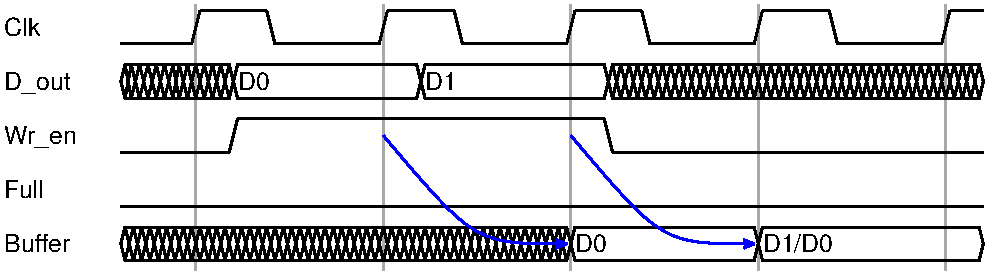
\includegraphics[width=1\textwidth]{timingdiagrams/write.pdf}
   \caption{Timing diagram for an FSL write operation}
   \label{fig:fsl-write}
\end{figure}

\section{Measurements and Discussion\label{sec:measurements}}
This section describes the results obtained from the experiments. To get consistent results, the timer was configured to measure only the actual calculation and not the communication with the operator. In the hardware accelerated solution the timer was started just before the operands were sent to the hardware IP core and stopped just after the final result could be read back.
%This is probably the most important part of the report. In here you must describe the what and how you measure. Describe any specific parts in the hardware architecture or the software that help you conduct measurements. You should use graphs or tables to present your results, such as Table \ref{tab:example} or \ref{tab:example2}, but do not forget to describe the measures and units in the columns or graph axis.

% Requires the booktabs if the memoir class is not being used
\begin{table}[htbp]
   \centering
   %\topcaption{Table captions are better up top} % requires the topcapt package
   \begin{tabular}{rrrrr} % Column formatting, @{} suppresses leading/trailing space
      \toprule
	N & GCD & Single processor	& Dual processor	& Hardware accelerated\\
      \midrule
      10	& 71 & 24978			& 12726			&1595\\
      30	& 3 & 1992704		&  928490		&100623\\
      50	& 6211 & 17097			& 9207			&2485\\
      70	& 128 & 108319		& 58745			&7688\\
     100	& 587 & 37876			&  21217		&5129\\
      \bottomrule
   \end{tabular}
   \caption{Performance numbers for the different implementations}
   \label{tab:Clockcycles}
\end{table}



\subsection{Performance}
The performance figures are presented in table~\ref{tab:Clockcycles}. In the single and dual processor solution the GCD calculation was done in software only. The results show that the dual processor solution takes just over half the time compared to the single processor solution in all datasets but one, where it takes slightly less than half. This was not suprising to us since each core can calculate the GCD for half the dataset independently, without having to wait for or synchronize with the other core until the end. The FSL transfers are included in the clock cycle counts, but the dual processor solution is still almost twice as fast. From this we can draw the conclusion that the Fast Simplex Link is very fast indeed. Using shared memory between the cores instead may yield even better performance, as no data would have to be exchanged at all.

The hardware accelerated solution is almost an order of magnitude faster than both the single and dual processor solution. The GCD calculation is moved completely into hardware. The software is only responsible for communication with the operator and communicating the operands and result with the hardware IP core. Even better performance would likely be obtained by hardware accelerating more parts, like the entire GCD for N numbers algorithm.

Table~\ref{tab:Clockcycles} shows the time taken (as measured in CPU clock cycles) to calculate the GCD for the sample data\cite{assignments}. The table shows that the time increases when the final GCD decreases. This is because of properties of the euclidean algorithm. The time required is proportional to the number of divisions required, or in its simplified version, the number of subtractions.

%How about compiler optimizations? 


\subsection{Device Utilization}
%Give the FPGA resources consumed by each of your solutions. Explain how these relate to each other -- e.g. whether a dual processor system has double the area of a single processor system and how do these relate to the hardware accelerated solution. Explain why or how using different algorithms influences or not the device utilization.
The Xilinx tools are capable of exporting hardware utilization numbers in great detail. A selection of these that were found interesting are presented in table~\ref{tab:Utilization}

\begin{table}[htbp]
  \centering
  % \topcaption{Table captions are better up top} % requires the topcapt package
  \begin{tabular}{lrrrr} % Column formatting, @{} suppresses leading/trailing space
    \toprule
    Name & Single processor & Dual processor & Hardware accelerated & Available \\
    \midrule
    CLB Flip-Flops & 1,684 & 2,499 & 1,812 & 18,224 \\ % Slice Registers
    LUTs used as logic & 2,092 & 3,222 & 2,352 & 9,112 \\
    LUTs used as memory & 152 & 301 & 187 & 2,176 \\ % RAM, dvs processorregister? samt skiftregister
    Occupied Slices & 962 & 1,411 & 992 & 2,278 \\
    16K block RAMs & 16 & 32 & 16 & 32 \\
    \bottomrule
  \end{tabular}
  \caption{Hardware utilization for the different implementations}
  \label{tab:Utilization}
\end{table}

\subsection{Power and Energy}
The power and energy usage numbers are presented in table~\ref{tab:Power}. The power has been estimated with the Xilinx XPower Analyser. The energy consumption has been calculated using formula~\eqref{eq:energy} where the frequency is 100 MHz. The result is measured in Watt-seconds, or Joules. For the energy consumption comparisons, the performance numbers for $N=30$ was used, as this had the longest run-time across all three implementations.

\begin{equation}
  \label{eq:energy}
  E = P \Delta t = P \cdot \frac{clock\ cycles}{frequency}
\end{equation}

The power consumption does not differ much between the implementations. The single processor implementation has the lowest power consumption. This was expected, since it has the least amount of hardware. The increase in power consumption when a second MicroBlaze core was added is surprisingly small. As with the hardware utilization, this is probably explained by the fact that a lot of the hardware is shared by the the processors. The power consumption in the hardware accelerated solution is only slightly higher than the uniprocessor solution. This was not surprising, since the hardware IP core is very small and simple.

There was however a significant difference in the energy consumption between the implementations. After reading the power consumption number, this was not unexpected since the energy consumption is proportional to the clock cycles used, as can be seen in formula~\eqref{eq:energy}. As the power is fairly constant between the implementations, the energy used by the hardware solution is an order of magnitude lower than the software implementations.

\begin{table}[htbp]
  \centering
  % \topcaption{Table captions are better up top} % requires the topcapt package
  \begin{tabular}{lrrr} % Column formatting, @{} suppresses leading/trailing space
    \toprule
    & Single processor  & Dual processor    & Hardware accelerated\\
    \midrule
    Power (W)   & 0.163         & 0.172         & 0.164\\

    Energy (mJ) & 3.25       & 1.60     & 0.165\\
    \bottomrule
  \end{tabular}
  \caption{Power and energy consumption for the different implementations calculated from the GCD for $N=30$ results}
  \label{tab:Power}
\end{table}

\section{Summary\label{sec:summary}}
It has become very clear during the sessions how software and hardware relate to each other in question of performance.
%In this part you briefly summarize your report. Continue with conclusions, lessons learned, unexpected results, unsolved problems or other issues that remain open. Relate back to the content of the course and explain whether or how the laboratory work helped you or not with understanding certain issues from the theoretical part.

\bibliographystyle{plain}
\bibliography{abibfile}

\end{document}  
